\documentclass[11pt]{article}
% Target journal: Evolutionary Human Sciences (Cambridge University Press),
% open access, IMRaD, author-date references, a short social-media summary, and
% an abstract. Drafted as a clean generic article; the EHS submission class and
% their exact front-matter fields can be slotted in once confirmed against the
% author guidelines. Manuscript source is TeX-only and compiles with pdflatex
% (project convention). ASCII only; no em dashes in prose.
%
% NUMBER PROVENANCE:
%  - Confirmatory core (C1 h^2, C2 repeatability, S, C3, H1-H3) and the two
%    exploratory analyses (within-era Moran's I, reproductive rate) are computed
%    on the CURRENT gene pipeline (commit c5a2f35) and validated (ehs_validate.py).
%  - Phenotype-validity supporting stats (variance decomposition, cross-team
%    travel, persistence, face validity) regenerated on the current genes
%    2026-07-01 and updated in-text (no stale figures remain).
% EHS SUBMISSION NOTES (Cambridge author instructions, retrieved 2026-07-01):
%  - Overleaf class 'cambridge-medium-template-class-file'
%    (overleaf.com/latex/templates/cambridge-medium-template-class-file/zshzqdxjjqkq);
%    drafted here as generic article, retarget to their class before submission.
%  - APA author-date citations; abstract <=200 words; main text <=8000 words;
%    <=8 display items; <=75 references; keywords >=3; title <12 words.
%  - Graphical abstract required (PNG >=900px) -- the h2 x S map can serve.
%  - Social-media summary <=120 characters (final draft only).
\usepackage[utf8]{inputenc}
\usepackage[T1]{fontenc}
\usepackage{lmodern}
\usepackage[margin=1in]{geometry}
\usepackage{booktabs}
\usepackage{amsmath}
\usepackage{graphicx}
\usepackage{parskip}
\usepackage{microtype}
\usepackage{authblk}
\usepackage[round,authoryear]{natbib}
\usepackage[hidelinks]{hyperref}
\setlength{\emergencystretch}{2em}

\title{\bfseries Heritability and selection of strategic traits in the NFL coaching tree}
\author[1]{Jon Williamson}
\affil[1]{Williamson Consulting Group. Correspondence: jonwilliamson@live.com}
\date{Draft \today}

\begin{document}
\maketitle

%% ----------------------------------------------------------------------------
\noindent\textbf{Social media summary.}
NFL coaching lineages inherit a mentor's system, not his success: what transmits
is largely not what wins.

\begin{abstract}
\noindent Human expertise is transmitted socially, and where learners have
identifiable teachers the transmission leaves a genealogy. We treat the National
Football League coaching tree as a cultural pedigree and, for a preregistered set
of ten standardized play-calling traits, estimate each trait's transmissibility
($h^{2}$, mentor-to-protege resemblance from a Bayesian parent-offspring model with
a measurement-error correction) and its selection ($S$, association with a coach's
wins above replacement). Every trait is a genuine, repeatable individual
characteristic (repeatabilities 0.34 to 0.58), yet transmissibility and selection
come apart. Schematic-identity traits transmit but do not win: shotgun $h^{2}=0.45$
(95\% HDI $[0.27,0.65]$) with $S=0.08$, and tempo similarly. Offensive aggression is
the mirror image, repeatable ($0.40$) and selected ($S=0.18$, $[0.08,0.27]$) yet not
transmitted ($h^{2}=-0.15$); a preregistered contrast confirms it is repeatable but
not heritable ($0.55$, $[0.24,0.87]$). Defensive aggression alone both transmits
($h^{2}=0.49$) and wins ($S=0.15$). The predicted negative heritability-fitness
relationship does not appear (Spearman $+0.32$, $[-0.54,0.69]$): rather than a
trade-off, transmission and selection are largely decoupled. Coaching lineages
propagate systems, not success, and the fitness-linked behavior spreads through a
channel a purely vertical lens would miss.
\end{abstract}

\smallskip
\noindent\textbf{Keywords:} cultural evolution; social learning; vertical
transmission; heritability; cultural fitness; sport.

\bigskip
\noindent\textbf{Preregistration.} The confirmatory analyses (C1--C3, hypotheses
H1--H3) and their decision rules were registered before any confirmatory quantity
was computed on the final measurement pipeline:
\href{https://doi.org/10.17605/OSF.IO/Y2KR5}{osf.io/y2kr5}
(\texttt{doi:10.17605/OSF.IO/Y2KR5}). We report the preregistered verdicts as they
fell, supported or not, and flag any deviation where it occurs.

\noindent\textbf{Data and code availability.} All data and code are public and
seed-fixed: \href{https://github.com/jwilliamson7/Coach_Tree}{github.com/jwilliamson7/Coach\_Tree}
and \href{https://github.com/jwilliamson7/Coach_WAR}{github.com/jwilliamson7/Coach\_WAR}
(the source of the WAR phenotype, pinned at commit \texttt{dffe2f1}). The full
pipeline runs from one command (\texttt{scripts/analysis/run\_ehs\_confirmatory.py}).

%% ----------------------------------------------------------------------------
\section{Introduction}
%% ----------------------------------------------------------------------------

Human skilled practice is transmitted socially, and where practitioners learn from
identifiable teachers the transmission leaves a genealogy. Coaching in the National
Football League (NFL) is an unusually legible case. Head coaches hire assistants,
assistants become coordinators, coordinators are promoted to head coach, and the
record of who worked under whom is documented season by season. The result is a
``coaching tree'': a directed network of mentor--protege ties along which styles of
play are widely believed to descend. Popular accounts speak of the Walsh tree or
the Belichick tree much as a breeder speaks of a bloodline, and NFL hiring leans
heavily on that pedigree logic, on the assumption that working under a successful
coach transfers both winning approaches and strategic expertise.

Cultural evolution treats socially learned behavior as a second inheritance system,
one that, like the genetic system, is transmitted, varies, and is subject to
selection \citep{cavallisforza1981, boydricherson1985, henrich2016}. Much of the
human capital that distinguishes experts, from surgeons to craftspeople to coaches,
is acquired by working under a more accomplished practitioner rather than from
books, so expertise descends along chains of apprenticeship. Measuring vertical
transmission in such chains is nonetheless hard: it requires observing the same
behavior in both teacher and learner, on a comparable scale, with the genealogy
known, and human pedigrees of behavior are seldom that legible. Professional sport
is an exception, because the record of who coached under whom is public and the
behavior itself, every play call, is logged.

Recent work has begun to treat sport tactics as a cultural-evolutionary system.
\citet{mesoudi2020}, in this journal, analyzed the cultural evolution of
association-football formations and showed that a managerial innovation spread
through strategic social learning among contemporaries, a \emph{horizontal}
diffusion that accelerated as the tactic proved successful. That study measured
transmission among peers and explicitly named transmission along mentor--protege
lineages, the \emph{vertical} channel, as open work. The present paper takes up
exactly that question, for a different sport. Cultural transmission theory
distinguishes vertical transmission, from a parent-like model to a learner, from
horizontal transmission among contemporaries, and the two need not carry the same
traits \citep{cavallisforza1981, boydricherson1985}. A coaching tree is an
unusually direct substrate for the vertical channel, because both the mentor's and
the protege's on-field behavior are observed and dated. As we will show, the
vertical and horizontal channels in coaching turn out to move \emph{different}
strategic traits, so the two studies are complementary halves of one picture.

To ask how faithfully behavior descends such a pedigree, we borrow the toolkit
quantitative genetics built for that decomposition. Two quantities anchor it.
Repeatability is the share of a trait's variance that is a stable property of the
individual rather than occasion-to-occasion noise, and it sets an upper bound on how
much of the trait can be transmitted at all. Heritability is the share actually
passed to descendants; in a parent-offspring design it is read directly from the
resemblance between parent and offspring phenotypes, with no need for an assumed
relatedness matrix \citep{falconermackay1996}. The same variance-partitioning logic
extends from classical pedigrees to repeated measures through the mixed-model animal
model \citep{wilson2010, nakagawa2010}, and dual-inheritance theory has long held
that it applies to culturally transmitted traits as well as genetic ones
\citep{cavallisforza1981}. What has been missing for culture is a system in which
both the pedigree and the phenotype are observed directly rather than inferred; the
coaching tree supplies one.

We use these tools to place each trait on two axes. The first is transmissibility,
the cultural analog of heritability $h^{2}$: how strongly a protege's own
head-coaching style resembles the style of the coach they apprenticed under. The
second is selection $S$: how strongly a trait covaries with success, measured here
as a coach's context-adjusted wins above replacement (WAR). In biological
populations the two are famously in tension. Fisher's fundamental theorem implies
that selection consumes the additive genetic variance of the traits most closely
tied to fitness, so those traits should be the \emph{least} heritable
\citep{fisher1930}. The prediction holds across taxa: \citet{mousseauroff1987}
found life-history traits, those nearest fitness, markedly less heritable than
morphological ones, and \citet{kruuk2000} report a rank correlation near $-0.8$
between the heritability of a suite of red-deer traits and their association with
fitness. Whether an analogous tension arises in a cultural system, where
inheritance is social learning rather than meiosis and the variance-depleting logic
of Fisher's theorem need not apply, is unknown.

The coaching tree is a favorable model system for the question. Every offensive and
defensive decision is recorded play by play, so a coach's tendencies can be measured
as deviations from what the game situation demands; the mentor-protege genealogy is
documented, so vertical transmission can be traced from a coach's coordinator
apprenticeship to their own head-coaching tenure; and coaching success has a
context-adjusted measure, wins above replacement, that separates a coach's
contribution from roster talent. Because a coordinator's later head-coaching behavior
is observed after and apart from the mentor's, the design is a genuine
between-person parent-offspring comparison rather than a coach correlated with
himself.

We ask a single organizing question: in the NFL coaching tree, are the strategic
traits that transmit the same traits that win? We separate strategy into two
families. \emph{Approach-to-scenarios} traits describe how aggressively a coach
attacks game situations (going for it on fourth down, passing in neutral
situations, throwing beyond the first-down marker, attempting two-point
conversions, and on defense loading the box, sending extra rushers, and playing man
coverage). \emph{Schematic-identity} traits describe the formational signature of a
team (how much it operates from shotgun, and how fast it plays). The split is
cleanest on offense; as we find, defensive ``aggression'' mixes an attitudinal and a
schematic component (Discussion). Our preregistered hypotheses were:
\begin{itemize}
  \item[H1.] Approach traits are more strongly \emph{selected} (predict WAR), while
  identity traits are more strongly \emph{inherited} (transmit down the tree).
  \item[H2.] Offensive aggression is a repeatable individual trait that is
  nonetheless not heritable: its within-coach repeatability clearly exceeds its
  transmissibility.
  \item[H3.] Across the ten sub-traits, heritability and selection are negatively
  related: the traits that transmit most strongly are not the ones that predict
  winning.
\end{itemize}
These predictions were registered before any confirmatory quantity was computed on
the final measurement pipeline (Section~\ref{sec:methods}). As reported below, the
data support a decoupling of transmission and selection but not the specific
negative trade-off of H3, and the picture is enriched by one trait, defensive
aggression, that both transmits and wins.

%% ----------------------------------------------------------------------------
\section{Materials and methods}\label{sec:methods}
%% ----------------------------------------------------------------------------

\subsection{Coaching phenotypes (``genes'')}
We construct standardized coach-season phenotypes from play-by-play data for the
2006--2024 NFL seasons (obtained through \texttt{nfl\_data\_py}; more than 600{,}000
plays). For each strategic decision we train a play-level expectation model
(gradient-boosted trees) on pre-play game context only, deliberately excluding
season, week, and coach identity, so the baseline reflects what an average coach
would do in identical circumstances and is time-invariant. A coach-season
phenotype is the average deviation of observed behavior from this expectation,
$\text{mean(actual)} - \text{mean(predicted)}$, standardized (z-scored) across the
coach-season panel; positive values denote more aggressive, faster, or more
shotgun-oriented play than context predicts. This residual construction isolates a
strategic tendency from forced circumstance: a coach who goes for it often only
because he is always trailing is not thereby aggressive.

The ten sub-traits are the residuals of ten play-level models (Table~\ref{tab:traits}):
four offensive-aggression decisions (going for it on fourth down, passing versus
running in neutral situations, targeting beyond versus short of the first-down
marker, and attempting a two-point conversion), two tempo behaviors (no-huddle use
and seconds between snaps), three defensive behaviors (defenders in the box, number
of pass rushers, and man versus zone coverage), and shotgun formation use. Each is a
gradient-boosted model on pre-play context (down, distance, field position, score,
clock, and environment), a classifier for the discrete decisions and a regressor for
the continuous ones (pace, box count, rushers). Situational context explains most of
the variance in each decision, leaving the residual we read as tendency: out of
sample the classifiers range from man coverage (AUC 0.71) and pass targeting (0.73)
up to fourth-down decisions (0.98), and the regressors explain from very little of
pass-rusher counts (R$^2$ 0.06, most of which is therefore left to tendency) to a
substantial share of pace and box count (R$^2$ 0.43). Candidate feature sets are
pruned by stability selection, and the categorical encoders, imputer, and dimension
reduction are fit on the training split only, so each coach-season is scored in
exactly the feature space the model learned rather than one re-estimated on its own
plays.

Every play is attributed to the head coach who led the team for that game, so a
within-season head-coaching change splits the season between the two coaches at the
game of the change. Coordinators are not assigned their own phenotype; the
phenotype is defined only at the head-coach level, so a play is attributed to one
coach and never to both a head coach and a coordinator at once. To keep a coach's
own tendencies out of the yardstick that measures them, expectation models are fit
with the scoring coach held out and with cross-fitting folds balanced across eras,
so each play is scored by a model that never trained on that coach.

Ten sub-traits are frozen for the primary analysis (Table~\ref{tab:traits}),
grouped into four gene-level composites (offensive aggression, tempo, defensive
aggression, and shotgun) that serve as labeled exemplars but are not counted as
independent points in the cross-trait test.

\begin{table}[t]
\centering
\caption{The ten frozen sub-traits and their four gene-level composites. The two
families are approach-to-scenarios (aggression) and schematic identity.}
\label{tab:traits}
\begin{tabular}{lll}
\toprule
Composite (family) & Sub-traits & Data window \\
\midrule
Offensive aggression (approach) & fourth-down, pass-heavy, deep-pass, two-point & 2006--2024 \\
Tempo (identity)                & no-huddle, pace                              & 2006--2024 \\
Defensive aggression (approach) & box-stacking, pass-rush                      & 2016--2024 \\
                                & man-coverage                                 & 2018--2024 \\
Shotgun (identity)              & shotgun                                      & 2006--2024 \\
\bottomrule
\end{tabular}
\end{table}

\subsection{Contemporary-group (era) adjustment}
Each phenotype is expressed as a deviation from its own season's league mean
(within-season demeaning) before any modeling. Because both a mentor's and a
protege's values are re-centered on their own seasons, league-wide drift is removed
exactly once and is not counted as transmission or selection. This is the single
era control, the cultural analog of the contemporary-group (herd-year-season)
adjustment used to estimate breeding values in the animal model; no further season
or era term enters the models. Coach WAR is already a within-season,
replacement-relative quantity (about 3\% between-season variance) and receives no
further adjustment.

\subsection{Measurement error and reliability}
Each coach-season phenotype is an estimate with a known sampling variance, computed
per sub-trait from the play-level variance divided by the squared play count and
rescaled to the standardized scale. This per-observation variance is carried
explicitly in the heritability (C1) and repeatability (C2) models, so both are
estimated for the latent trait rather than its noisy observation. Composite genes
propagate their components' sampling variance; component reliabilities are estimated
with a DerSimonian--Laird random-effects decomposition \citep{dersimonian1986}.

\subsection{C1: transmissibility ($h^{2}$)}
A coordinator-to-head-coach transition pairs two different coaches. The outcome is
the protege's own phenotype once they became a head coach; the predictor is the
phenotype of the head coach they apprenticed under, measured on that mentor's team
over the seasons the protege served there as a coordinator. Each coach contributes
at most one transition per coordinator role (the most recent coordinator stint
preceding a head-coaching stint), which avoids pseudo-replication. Because the
phenotype is head-coach-level, this design measures whether the head-coaching style
a coach apprenticed under predicts that coach's own later style; it is a
between-person parent-offspring comparison, not a coordinator's own trait.

We estimate $h^{2}$ with a Bayesian multilevel parent-offspring model fit at the
coach-season grain \citep{wilson2010, nakagawa2010}. For protege $i$, a latent
mentor level $m_i$ and a latent own level $a_i$ are linked by
\begin{equation}
  a_i = \alpha + \beta\, m_i + \varepsilon_i, \qquad \varepsilon_i \sim \mathrm{Normal}(0,\sigma_a),
\end{equation}
and each individual mentor-overlap season $x_{ij}$ and protege head-coaching season
$y_{ik}$ loads on the corresponding latent level with a variance that combines a
shared true within-coach season-to-season component $\tau^2$ and the known
measurement variance of that observation:
\begin{equation}
  x_{ij}\sim\mathrm{Normal}\!\big(m_i,\ \sqrt{\tau^2+\mathrm{se}_{ij}^2}\big), \qquad
  y_{ik}\sim\mathrm{Normal}\!\big(a_i,\ \sqrt{\tau^2+\mathrm{se}_{ik}^2}\big).
\end{equation}
Modeling individual seasons rather than pre-averaging lets the mentor predictor
enter as a latent variable carrying its measurement variance, an errors-in-variables
correction for the attenuation that predictor noise would otherwise cause. The
transmissibility is the parent-offspring regression slope at the coach-season
grain,
\begin{equation}
  h^{2} \;=\; \frac{\beta\,\sigma_m^2}{\sigma_m^2+\tau^2}
        \;=\; \beta_{\text{latent}}\times \text{repeatability},
  \label{eq:h2}
\end{equation}
which is bounded above by the mentor repeatability $\sigma_m^2/(\sigma_m^2+\tau^2)$:
a trait cannot transmit more faithfully than it is a stable trait to begin with.
Because a mentor transmits a whole style rather than half a genome, the slope
itself is the transmissibility, with no Mendelian doubling. Priors are
$\mathrm{Normal}(0,1)$ on the intercept and slope (phenotypes are z-scored) and
half-$\mathrm{Normal}(0,1)$ on the variance components; sampling uses four chains
with 2000 post-warmup draws each, a non-centered parameterization, and target
diagnostics $\hat{R}\le 1.01$ and bulk effective sample size $>400$ (met for every
fit). As robustness checks the slope is refit with a mentor varying intercept and,
in a frequentist version, with mentor-clustered standard errors.

\subsection{C2: repeatability}
Per-trait repeatability is a Bayesian variance-components intraclass correlation on
the full head-coach coach-season panel, with the per-season measurement variance
carried as an explicit level so the ratio is the latent-trait repeatability,
$\sigma_{\text{between}}^2/(\sigma_{\text{between}}^2+\sigma_{\text{within}}^2)$. It
is the ceiling for $h^{2}$; because heritability cannot exceed repeatability, we
report $P(h^{2}>\text{repeatability})$ per trait, a value near one flagging a
specification problem rather than a substantive result.

\subsection{Selection ($S$)}
Selection $S$ is the era-adjusted, inverse-variance-weighted correlation of a trait
with Coach WAR: within-season demean the standardized gene and WAR, weight each
coach-season by its games-based WAR precision, and take the coach-clustered
weighted correlation. Single-season WAR is noisy, and because mean-zero noise in
the outcome attenuates a correlation rather than inflating it, this estimate is a
conservative floor. WAR is drawn from the sibling Coach\_WAR repository at commit
\texttt{dffe2f1} \citep{williamson2026war}.

\subsection{C3 and decision rules}
For the ten sub-traits we assemble the pair ($h^{2}$, $S$) and compute their
Spearman rank correlation with a 95\% bootstrap interval that resamples the traits
and draws $h^{2}$ from its posterior and $S$ from its bootstrap. The rank form is
the established test of the heritability-fitness relationship in quantitative
genetics \citep{mousseauroff1987, kruuk2000}. Each hypothesis is judged by one
pre-specified interval rule. H1 is supported if the approach family's mean $S$
exceeds the identity family's and the identity family's mean $h^{2}$ exceeds the
approach family's, each difference with a 95\% interval excluding zero. H2 is
supported if (aggression repeatability minus aggression $h^{2}$) has a 95\%
interval excluding zero. H3 is supported if the Spearman correlation is negative
with a 95\% bootstrap interval excluding zero.

\subsection{Exploratory analyses}
Two analyses are declared exploratory and corrected among themselves under a
Benjamini--Hochberg false-discovery rate \citep{benjamini1995}, separately from the
confirmatory tests. The first is a within-era Moran's $I$ on the mentor network (an
undirected, row-normalized adjacency of mentor--protege ties, with a permutation
null that shuffles trait labels only within career-midpoint era blocks)
\citep{moran1950}. The second is reproductive fitness as an exposure-normalized
rate: head-coaching offspring (proteges who themselves became head coaches) per
head-coaching season, with a minimum-exposure floor, together with the test of
whether coach quality predicts that rate net of exposure.

\subsection{Software}
Analyses are in Python; the Bayesian models use PyMC. The pipeline is seed-fixed and
runs from a single command.

%% ----------------------------------------------------------------------------
\section{Results}
%% ----------------------------------------------------------------------------

\subsection{The phenotypes are repeatable coach traits}
Before asking how a trait transmits or whether it wins, we confirm it is a stable
individual characteristic rather than a team artifact. Every trait is repeatable:
the latent-trait repeatabilities (Table~\ref{tab:main}) range from 0.34
(pass-heavy) to 0.58 (fourth-down), all clearly above zero, so each phenotype
carries substantial stable between-coach signal net of measurement noise. This is
the quantitative-genetics prerequisite for a meaningful heritability: a trait must
be repeatable before it can be transmissible.

Three companion analyses corroborate that the genes belong to the coach rather than
the team or its roster (Table~\ref{tab:validity}). First, a one-way variance
decomposition attributes far more of each gene's variance to coach identity than to
team identity (for composite offensive aggression, 0.50 versus 0.14). Because
$\eta^2$ inflates mechanically with the number of groups, and a coach maps to far
more levels than a team, we benchmark each against a cardinality-matched
label-permutation null: the coach excess over its null is about 0.29 against 0.08 for
team, so the coach signal is roughly three times larger, and the same ordering holds
for every gene. Second, when coaches change teams their tendencies travel with them:
across the 32 coaches who moved, composite offensive aggression at the new team
tracks the gene they showed at the old one ($r=0.55$, 95\% CI $[0.29,0.73]$, on the
era-adjusted gene), and in a mover regression the coach's prior-team gene carries
$\beta=0.54$ ($[0.26,0.88]$) net of the destination's pre-arrival identity. Third,
the genes persist from season to season (composite offensive aggression lag-1
$r=0.50$, with its four components between 0.43 and 0.55). At only 32 movers the
travel test is imprecise for any single gene, which is why the composite, which
averages out component sampling noise, travels most cleanly.

\begin{table}[t]
\centering
\caption{The offensive genes are coach traits. One-way variance shares (coach, team,
season; marginal $\eta^2$, which need not sum to one because coach and team are
confounded), cross-team travel (era-adjusted across-team correlation among the 32
movers, 95\% CI), and year-to-year persistence (lag-1 correlation between consecutive
coach-seasons; computed for the aggression genes).}
\label{tab:validity}
\begin{tabular}{lccccc}
\toprule
Gene & coach $\eta^2$ & team $\eta^2$ & season $\eta^2$ & travel $r$ [95\% CI] & persist.\ $r$ \\
\midrule
Composite offensive aggression & 0.50 & 0.14 & 0.18 & 0.55 $[0.29,0.73]$ & 0.50 \\
\quad fourth-down & 0.51 & 0.07 & 0.26 & 0.09 $[-0.24,0.42]$ & 0.53 \\
\quad pass-heavy  & 0.49 & 0.18 & 0.08 & 0.32 $[-0.03,0.60]$ & 0.55 \\
\quad deep-pass   & 0.44 & 0.12 & 0.05 & 0.17 $[-0.20,0.51]$ & 0.46 \\
\quad two-point   & 0.44 & 0.09 & 0.17 & 0.30 $[0.04,0.60]$ & 0.43 \\
Shotgun & 0.57 & 0.12 & 0.48 & 0.28 $[-0.18,0.68]$ & -- \\
Tempo   & 0.52 & 0.11 & 0.07 & 0.48 $[-0.11,0.82]$ & -- \\
\bottomrule
\end{tabular}
\end{table}

Together with the repeatabilities, these lines establish that the phenotypes are
stable properties of the coach rather than artifacts of a roster, the prerequisite
for treating them as heritable-eligible traits.

\subsection{Transmissibility and selection come apart}
Table~\ref{tab:main} reports, for each trait, the preregistered transmissibility
$h^{2}$ (C1), repeatability (C2), and selection $S$. Two facts stand out. First,
transmissibility varies sharply across traits that are all similarly repeatable:
the schematic-identity genes transmit strongly (shotgun $h^{2}=0.45$, 95\% HDI
$[0.27,0.65]$; no-huddle $0.30$, $[0.09,0.51]$) as does defensive aggression
($0.49$, $[0.13,0.85]$), while offensive aggression does not transmit at all
($-0.15$, $[-0.46,0.12]$). Second, selection follows a nearly opposite ordering:
the approach components predict WAR (offensive aggression $S=0.18$, $[0.08,0.27]$;
defensive aggression $0.15$, $[0.03,0.27]$; pass-heavy $0.16$; pass-rush $0.17$)
while the identity genes do not (shotgun $0.08$, $[-0.03,0.17]$; tempo $0.03$). The
frequentist mentor-clustered slopes and the mentor varying-intercept refits agree
with the Bayesian $h^{2}$ (for example shotgun clustered slope $0.47$, $p<0.001$;
defensive $0.61$, $p=0.03$; offensive aggression $-0.03$, $p=0.85$).
Figure~\ref{fig:forest} plots each trait's $h^{2}$ against its repeatability ceiling
and makes the pattern legible at a glance.

\begin{figure}[t]
\centering
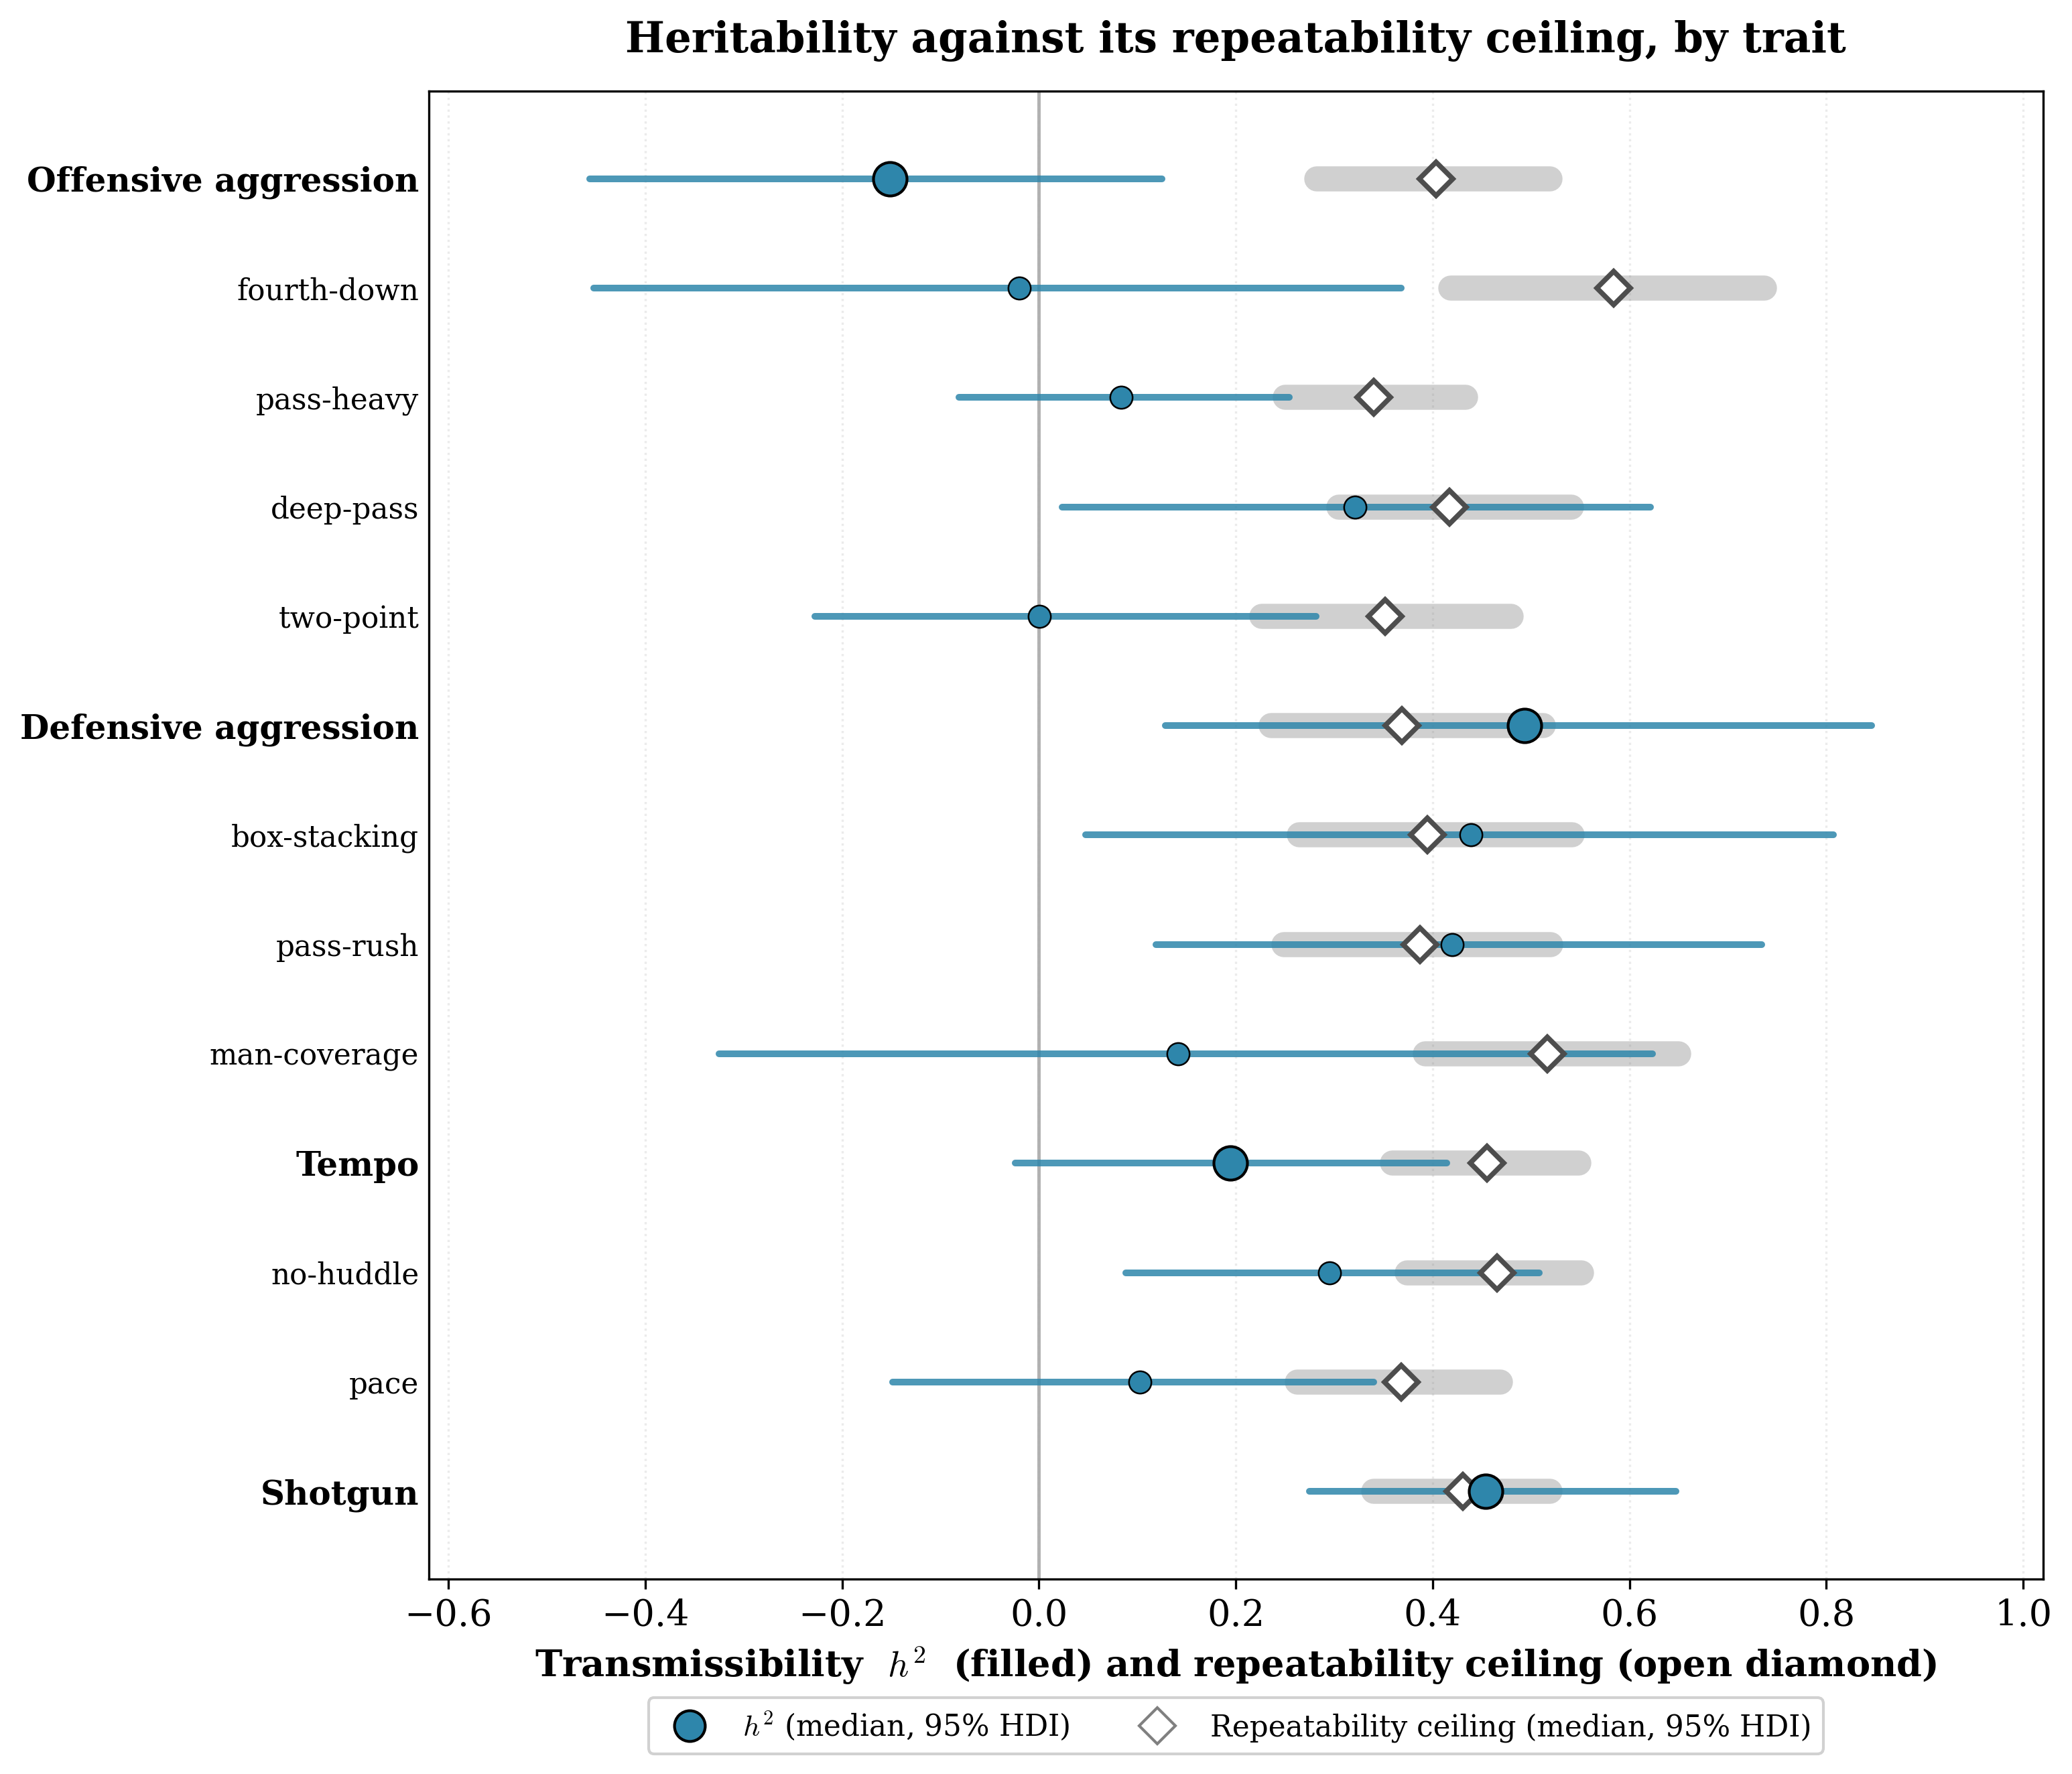
\includegraphics[width=0.92\textwidth]{../../visualizations/performance/ehs_heritability_forest.png}
\caption{Transmissibility ($h^{2}$, filled points with 95\% HDIs) against its
repeatability ceiling (open diamond, median; gray band, repeatability 95\% HDI) for
every trait, grouped by gene and colored by family. A heritability cannot exceed its
repeatability in the population; because $h^{2}$ and repeatability are estimated from
separate models with wide posteriors, their medians can cross for traits that
transmit near the ceiling, but every $h^{2}$ point falls within the repeatability's
credible interval (the posterior contrast $P(h^{2}>\text{repeatability})$ is 0.5 to
0.75 for these, that is $h^{2}\approx$ repeatability). Offensive aggression and its
components are repeatable but have $h^{2}$ indistinguishable from zero, a clean gap
($P=0.00$), the preregistered repeatable-but-not-heritable pattern (H2); schematic
identity and the defensive front transmit near their ceiling.}
\label{fig:forest}
\end{figure}

\begin{table}[t]
\centering
\caption{Transmissibility ($h^{2}$, C1), repeatability (C2), and selection ($S$)
for the four composites and the ten sub-traits. $h^{2}$ and repeatability are
posterior medians with 95\% HDIs; $S$ is the era-adjusted inverse-variance-weighted
correlation with WAR with a 95\% coach bootstrap CI. All C1/C2 fits met
$\hat{R}\le1.01$ and bulk ESS $>400$.}
\label{tab:main}
\begin{tabular}{llll}
\toprule
Trait & $h^{2}$ & repeatability & $S$ \\
\midrule
\textit{Offensive aggression} & $-0.15$ $[-0.46,0.12]$ & $0.40$ $[0.28,0.52]$ & $+0.18$ $[0.08,0.27]$ \\
\quad fourth-down   & $-0.02$ $[-0.45,0.37]$ & $0.58$ $[0.42,0.74]$ & $+0.04$ $[-0.05,0.13]$ \\
\quad pass-heavy    & $+0.08$ $[-0.08,0.25]$ & $0.34$ $[0.25,0.43]$ & $+0.16$ $[0.04,0.27]$ \\
\quad deep-pass     & $+0.32$ $[0.02,0.62]$  & $0.42$ $[0.30,0.54]$ & $+0.09$ $[0.00,0.17]$ \\
\quad two-point     & $+0.00$ $[-0.23,0.28]$ & $0.35$ $[0.23,0.48]$ & $-0.02$ $[-0.11,0.07]$ \\
\textit{Tempo}      & $+0.19$ $[-0.02,0.41]$ & $0.45$ $[0.36,0.55]$ & $+0.03$ $[-0.07,0.14]$ \\
\quad no-huddle     & $+0.30$ $[0.09,0.51]$  & $0.47$ $[0.37,0.55]$ & $-0.02$ $[-0.11,0.08]$ \\
\quad pace          & $+0.10$ $[-0.15,0.34]$ & $0.37$ $[0.26,0.47]$ & $+0.07$ $[-0.04,0.19]$ \\
\textit{Defensive aggression} & $+0.49$ $[0.13,0.85]$ & $0.37$ $[0.24,0.51]$ & $+0.15$ $[0.03,0.27]$ \\
\quad box-stacking  & $+0.44$ $[0.05,0.81]$  & $0.39$ $[0.26,0.54]$ & $+0.06$ $[-0.04,0.16]$ \\
\quad pass-rush     & $+0.42$ $[0.12,0.73]$  & $0.39$ $[0.25,0.52]$ & $+0.17$ $[0.04,0.29]$ \\
\quad man-coverage  & $+0.14$ $[-0.33,0.62]$ & $0.52$ $[0.39,0.65]$ & $+0.13$ $[-0.01,0.28]$ \\
\textit{Shotgun}    & $+0.45$ $[0.27,0.65]$  & $0.43$ $[0.34,0.52]$ & $+0.08$ $[-0.03,0.17]$ \\
\bottomrule
\end{tabular}
\end{table}

\subsection{The heritability by selection map and the preregistered verdicts}
Placing the four composites in $h^{2}\times S$ space (Figure~\ref{fig:map}) makes
the structure visible. Offensive aggression sits in the adaptive-but-personal
corner (selected, not heritable); shotgun and tempo sit in the heritable-but-neutral
corner (transmitted, not selected); defensive aggression sits alone in the
adaptive-and-heritable corner. The two axes are close to orthogonal.

\begin{figure}[t]
\centering
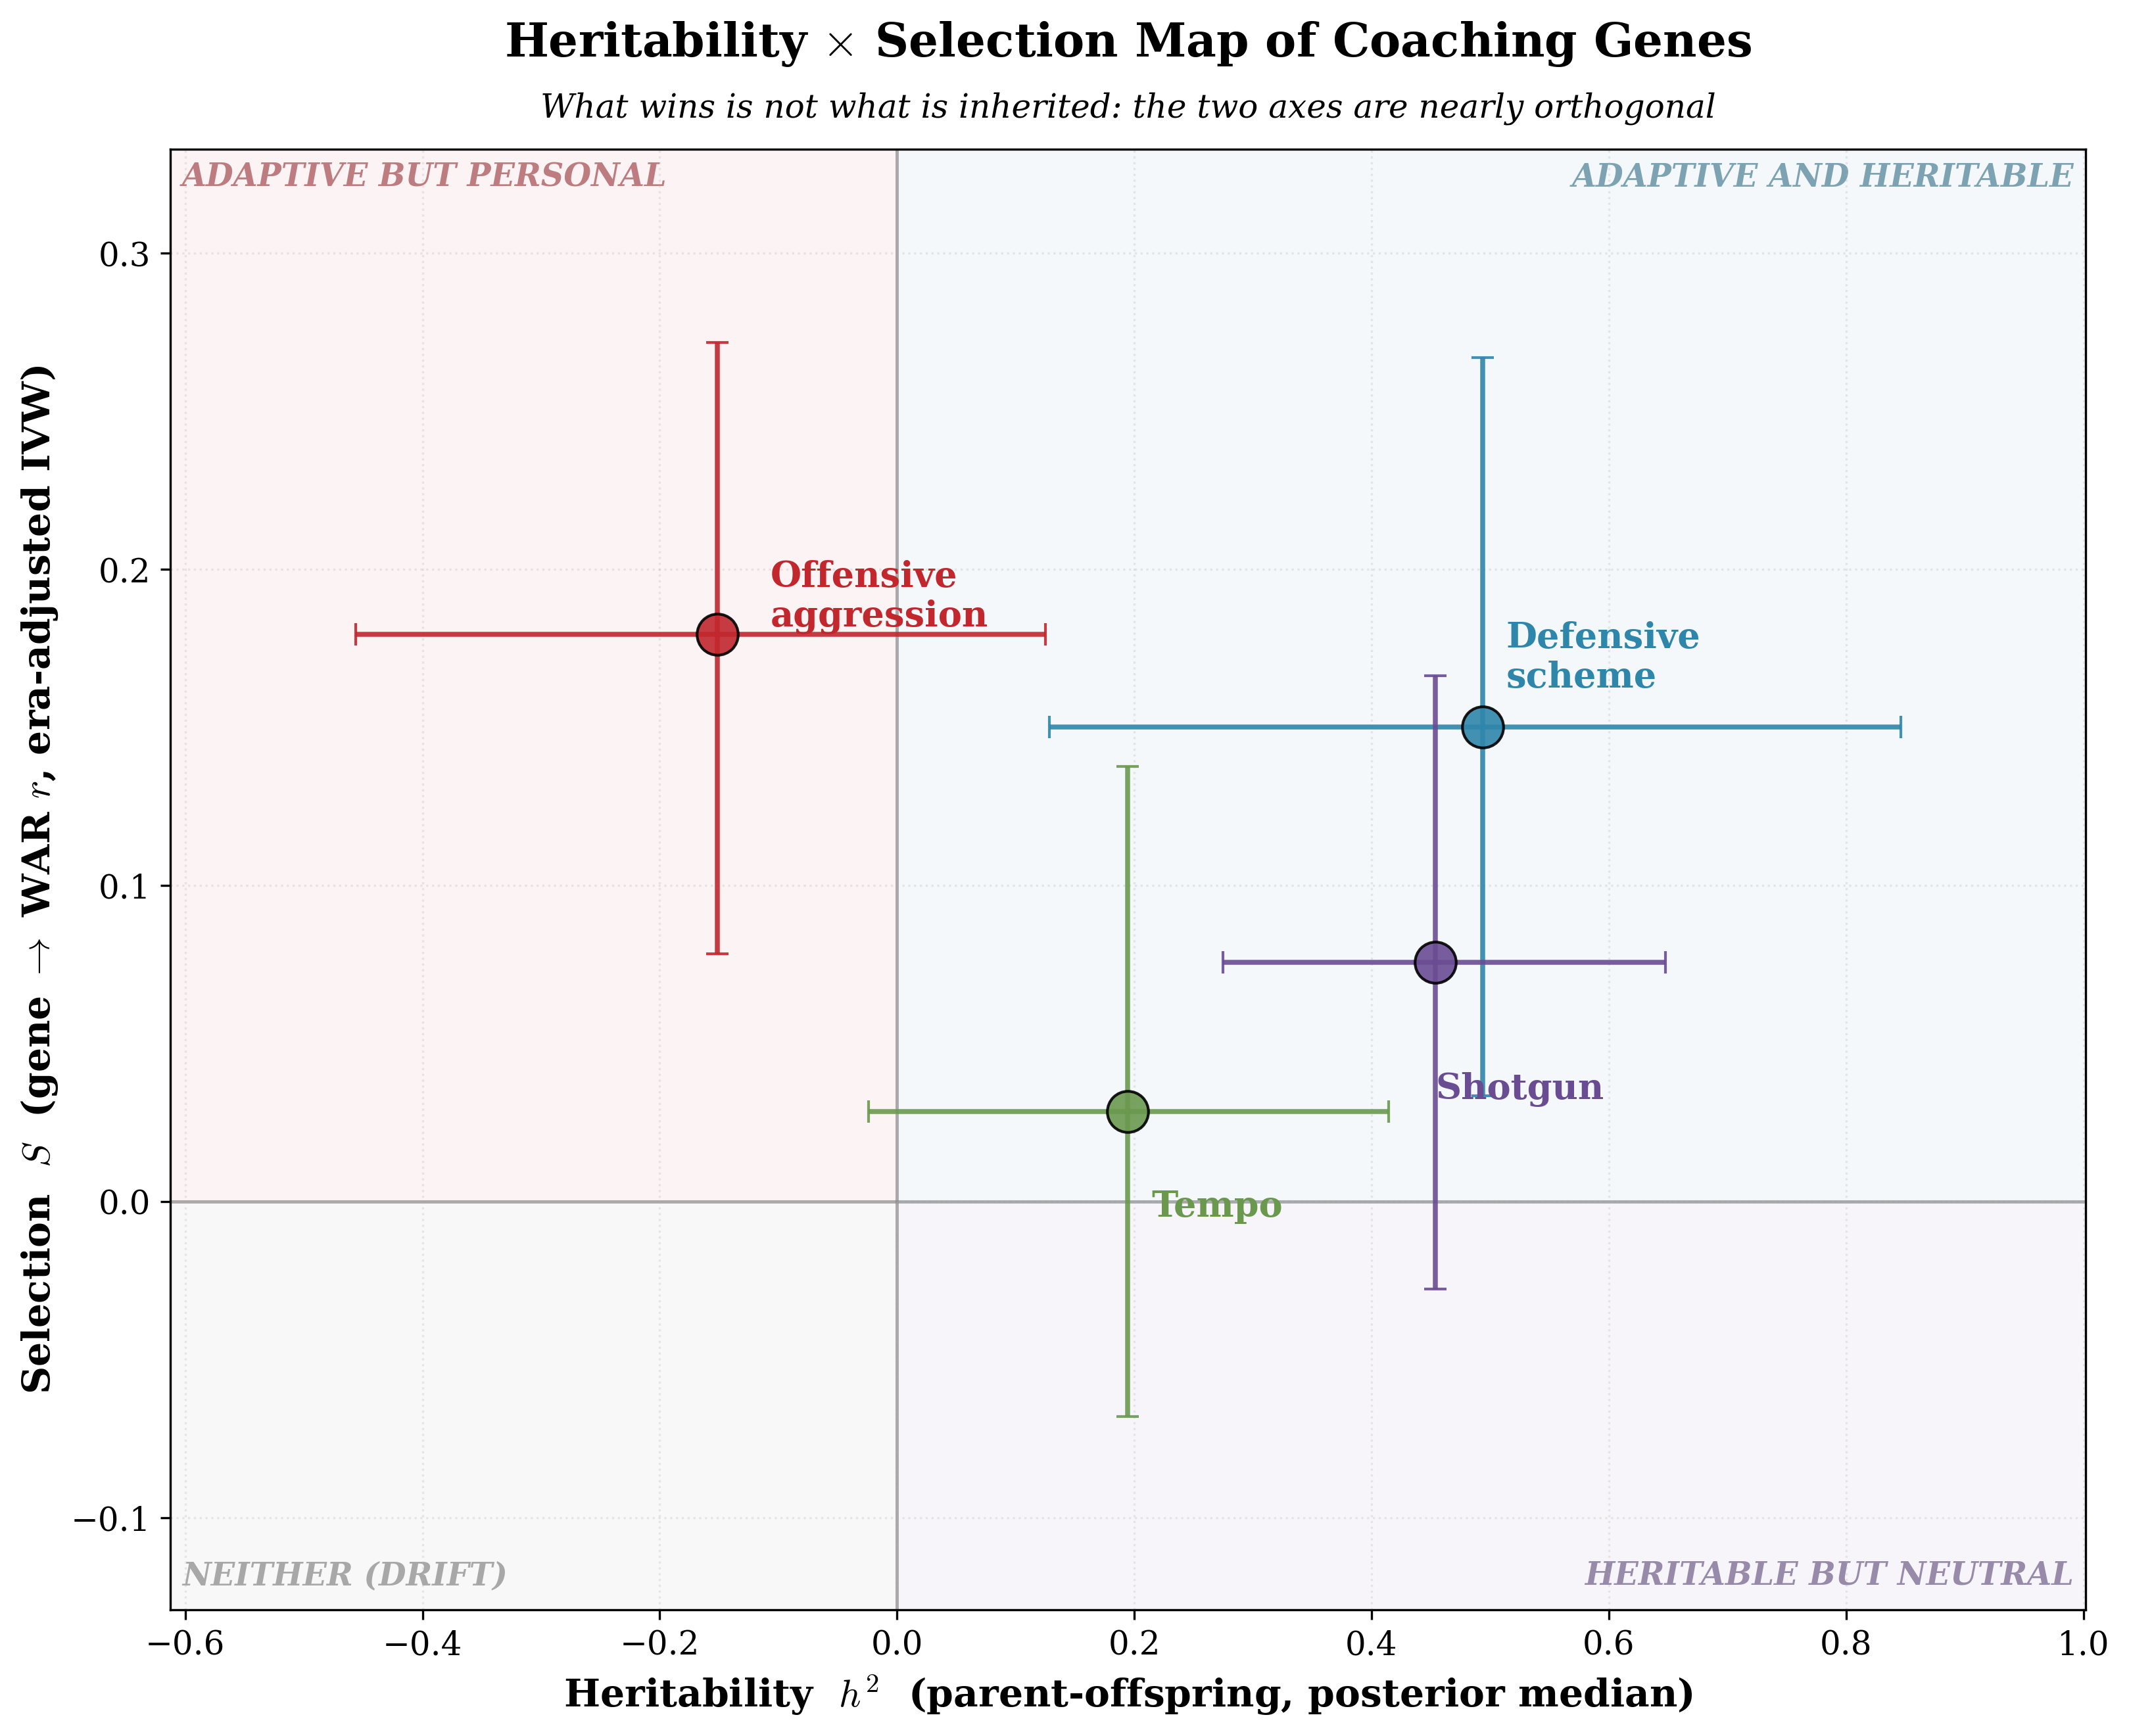
\includegraphics[width=0.86\textwidth]{../../visualizations/performance/gene_fitness_heritability_map.png}
\caption{Heritability ($h^{2}$, C1 posterior median) versus selection ($S$,
era-adjusted inverse-variance-weighted gene-WAR correlation) for the four
gene-level composites, with 95\% intervals on both axes. Offensive aggression is
adaptive but personal; shotgun and tempo are heritable but neutral; defensive
aggression is both. The axes are nearly independent.}
\label{fig:map}
\end{figure}

The three preregistered decision rules resolve as follows.

\textbf{H2 is supported.} Offensive aggression is repeatable ($0.40$) but not
heritable ($h^{2}=-0.15$); the preregistered contrast, repeatability minus $h^{2}$,
is $0.55$ with a 95\% HDI of $[0.24,0.87]$, excluding zero, and $P(h^{2}>\text{
repeatability})=0.00$. Offensive aggression is a real, stable, personal trait that
does not pass down the tree. The contrast behaves as the prereg intended
elsewhere too: for the traits that transmit near their ceiling (shotgun, defensive
aggression, box-stacking, pass-rush) $h^{2}$ and repeatability are statistically
indistinguishable ($P(h^{2}>\text{repeatability})$ between 0.5 and 0.75, each
$h^{2}$ inside the repeatability's credible interval), so the apparent crossings in
Figure~\ref{fig:forest} are estimation noise near the ceiling, not violations of the
bound.

\textbf{H1 is not supported as a conjunction, though its selection half holds.} The
approach family is more selected than the identity family (mean-$S$ difference
$+0.11$, 95\% interval $[0.01,0.22]$, excluding zero), but the identity family is
not reliably more heritable than the approach family (mean-$h^{2}$ difference
$+0.16$, $[-0.12,0.43]$, including zero). The heritability half fails for a
substantive reason: defensive aggression is an approach trait that is nonetheless
highly heritable ($h^{2}=0.49$), so the approach family does not have uniformly low
transmissibility.

\textbf{H3 is not supported.} Across the ten sub-traits the Spearman correlation
between $h^{2}$ and $S$ is $+0.32$ with a 95\% bootstrap interval of $[-0.54,0.69]$
(Figure~\ref{fig:scatter}): the point estimate is positive, the opposite of the
predicted negative trade-off, and the interval spans zero. The biological
heritability-fitness trade-off does not replicate here.

\begin{figure}[t]
\centering
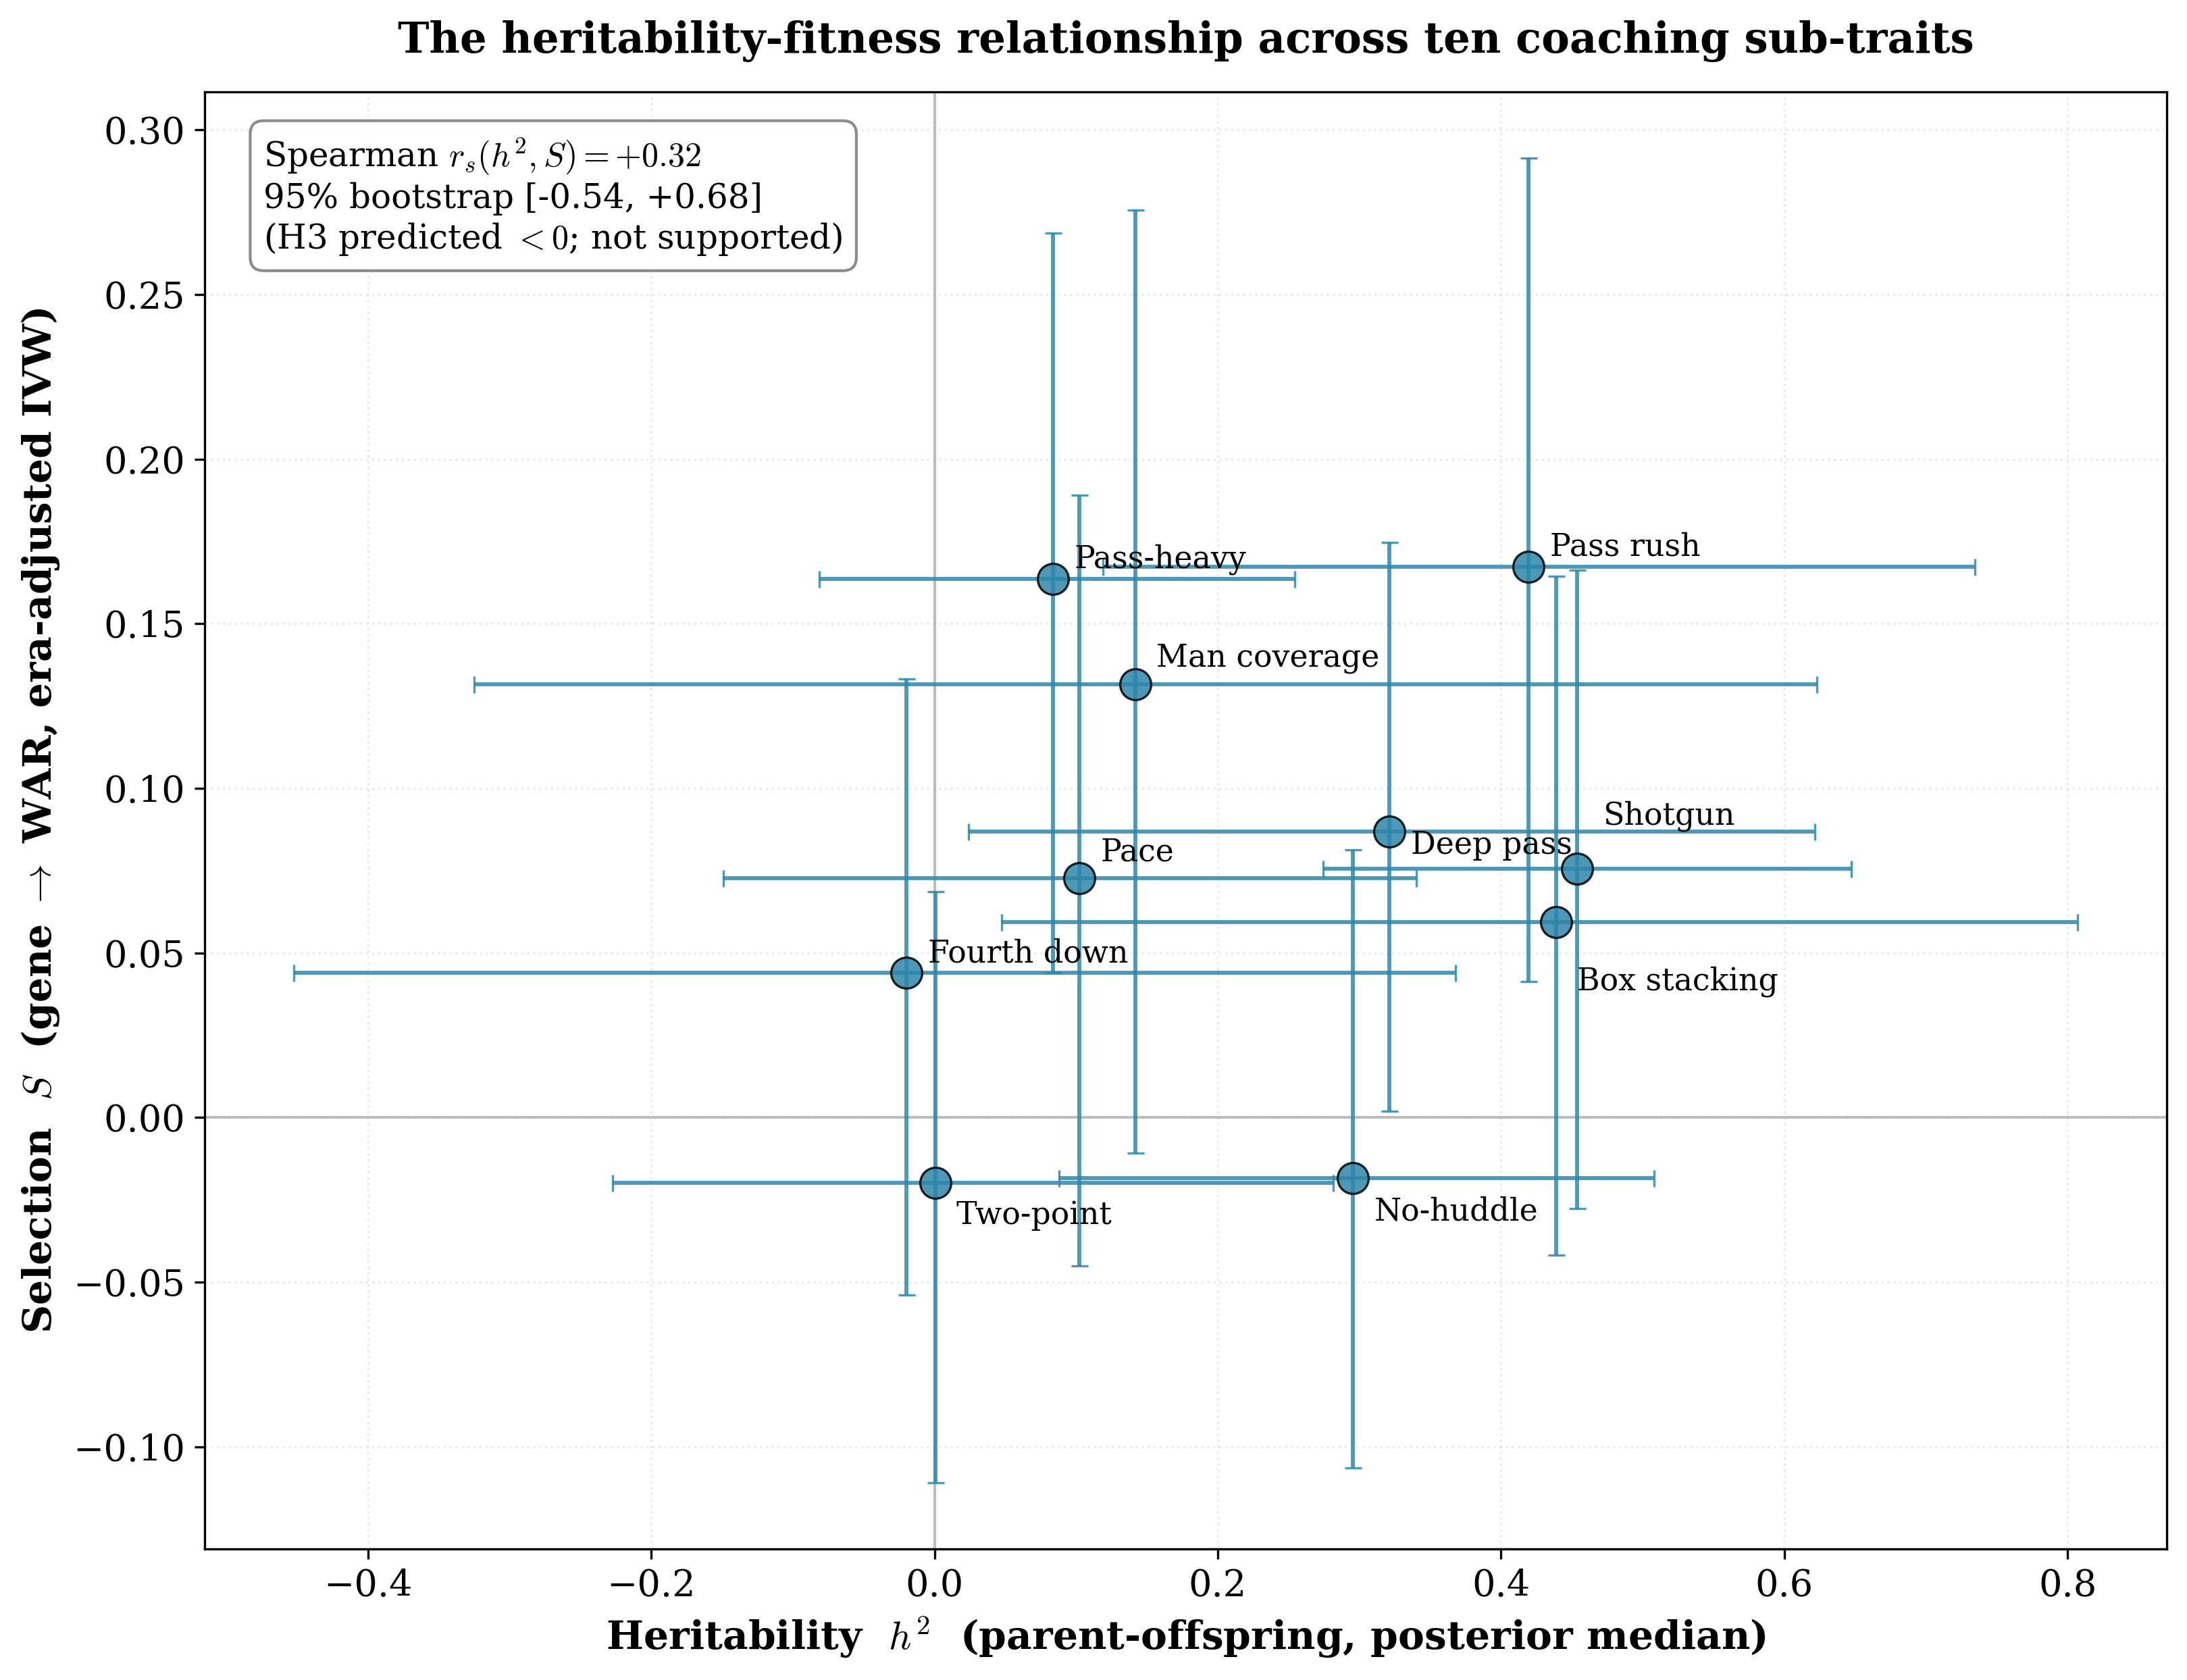
\includegraphics[width=0.9\textwidth]{../../visualizations/performance/ehs_cross_trait_h2_S.png}
\caption{The cross-trait heritability-fitness relationship, the cultural analog of
the wild-population test of \citet{mousseauroff1987} and \citet{kruuk2000}: each of
the ten sub-traits placed by transmissibility $h^{2}$ and selection $S$, with 95\%
intervals (a single colour throughout; the approach-versus-identity contrast is
drawn in the text, not by segmenting the figure). The Spearman rank correlation (H3)
is $+0.32$ ($[-0.54,0.69]$), not the predicted negative, so the two axes are
decoupled rather than traded off.}
\label{fig:scatter}
\end{figure}

Taken together, the verdicts describe a \emph{decoupling} rather than a trade-off.
Transmission and selection are close to independent across coaching traits, with
two clean archetypes, inherited-but-neutral identity (shotgun, tempo) and
selected-but-personal offensive aggression, and one trait, defensive aggression,
that occupies the both corner and is chiefly responsible for the absence of a clean
negative relationship.

\subsection{Exploratory: network signal and reproductive success}
Two exploratory analyses, corrected among themselves under a Benjamini--Hochberg
false-discovery rate, round out the picture; neither is confirmatory.

First, phylogenetic signal on the mentor network (Table~\ref{tab:moran},
Supplementary material). Moran's
$I$, the network analog of the tendency of related individuals to resemble one
another, is positive for the schematic and defensive genes and essentially zero for
offensive aggression (defensive aggression $I=0.21$, within-era permutation
$p=0.002$; tempo $0.12$, $p=0.008$; shotgun $0.08$, $p=0.04$; offensive aggression
$-0.01$, $p=0.52$). Under the exploratory correction the defensive and tempo signals
survive. The pattern mirrors the transmission results exactly: network-adjacent
coaches resemble one another in the traits that transmit and not in the trait that
does not, a second and independent line of evidence for the same decoupling.

Second, reproductive success, the other face of fitness (Figure~\ref{fig:repro}).
Counting a mentor's distinct proteges who themselves became head coaches, the
distribution is heavy-tailed: across 463 head coaches the Gini coefficient is 0.66
and the most prolific decile produced 43\% of all head-coaching descendants, with
Marty Schottenheimer and Bill Parcells (13 each), Bill Belichick (12), and Andy Reid
(11) at the top. Reproductive success tracks career WAR ($r=0.36$), but the link runs
through longevity rather than per-season quality: offspring count correlates 0.71
with seasons coached, and net of tenure the exposure-normalized rate (offspring per
head-coaching season) is essentially unrelated to quality (partial $r=0.09$). A
coach's ecological fitness (winning) and reproductive fitness (descendants) are thus
only weakly linked, and through survival: coaches shape the league less by winning in
any given season than by lasting long enough to send many proteges into
head-coaching chairs, carrying their schematic identity, though not their competitive
edge, with them.

\begin{figure}[t]
\centering
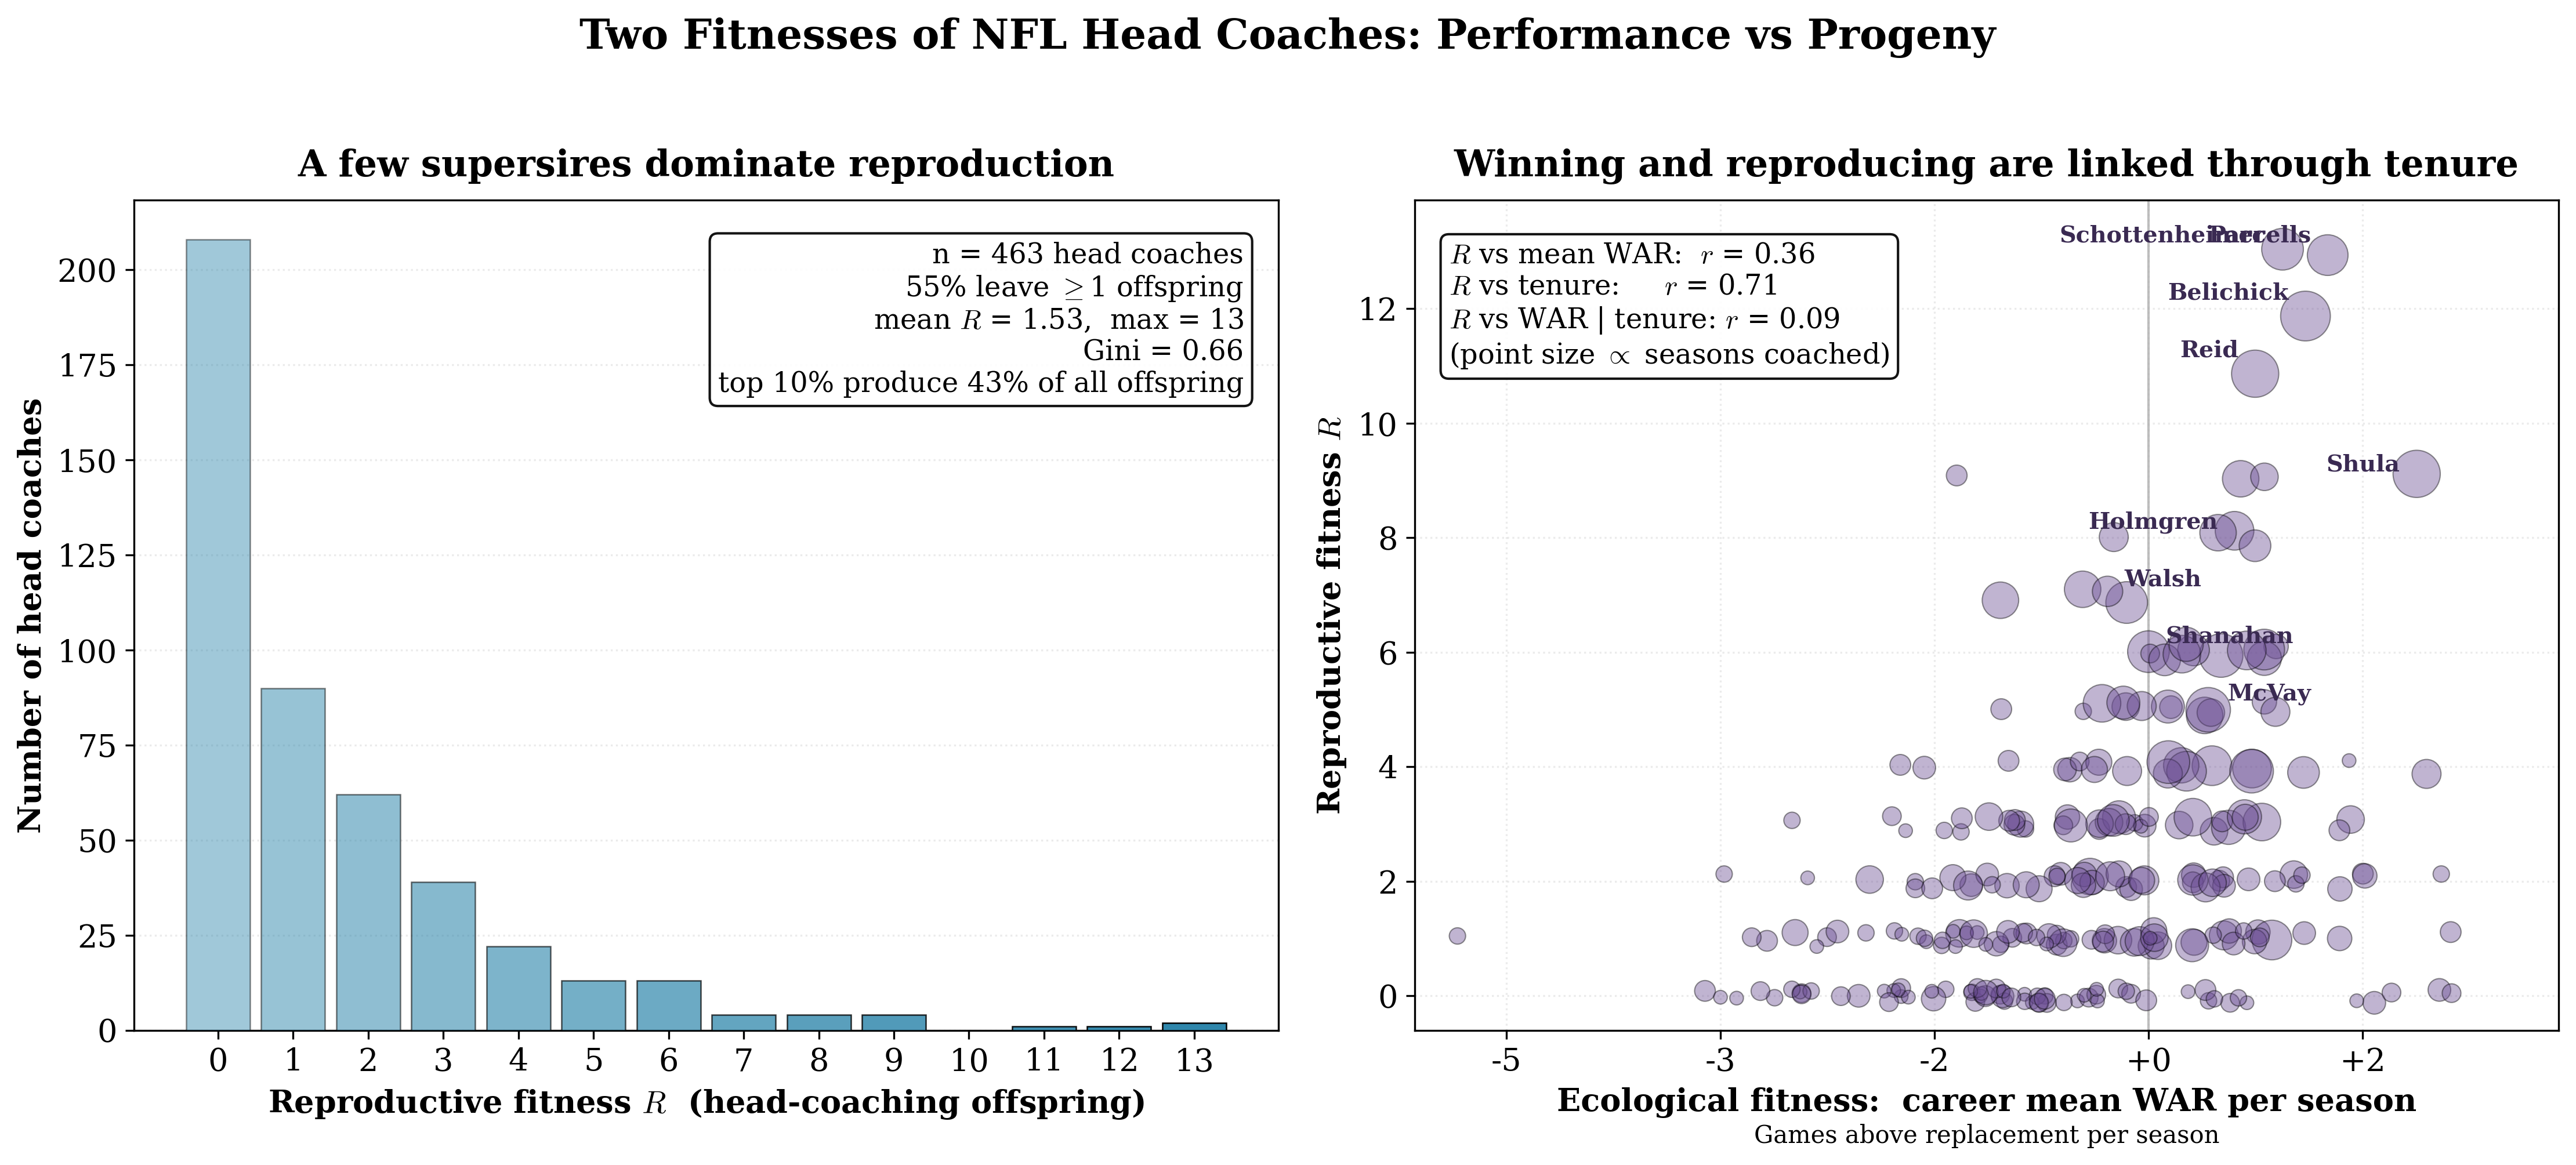
\includegraphics[width=0.92\textwidth]{../../visualizations/performance/reproductive_fitness.png}
\caption{Two fitnesses of NFL head coaches. Left: the distribution of reproductive
fitness (number of head-coaching proteges) is heavy-tailed (Gini 0.66; top decile
produces 43\% of all descendants). Right: ecological fitness (career mean WAR per
season) versus reproductive fitness, point size proportional to seasons coached; the
positive raw association ($r=0.36$) is carried by tenure (offspring versus seasons
coached $r=0.71$), and net of tenure quality barely predicts offspring (partial
$r=0.09$).}
\label{fig:repro}
\end{figure}

%% ----------------------------------------------------------------------------
\section{Discussion}
%% ----------------------------------------------------------------------------

\subsection{Decoupling, not a trade-off}
We set out to test whether the traits that transmit down a coaching lineage are the
traits that win, expecting the negative heritability-fitness relationship familiar
from biological populations. That specific trade-off did not appear. Instead,
transmission and selection are largely \emph{decoupled}: across ten strategic
traits the two axes are close to orthogonal (cross-trait Spearman $+0.32$, interval
spanning zero), not negatively related. The result is not the absence of structure
but a different structure. Two archetypes are clean. Schematic-identity traits,
shotgun and tempo, are transmitted faithfully ($h^{2}$ up to $0.45$) yet carry no
detectable fitness consequence ($S\approx0$): in evolutionary terms they behave
like heritable but selectively neutral markers \citep{kimura1968}, tags of lineage
that ride along with apprenticeship rather than with winning. Offensive aggression
is the mirror image, a repeatable and selected but non-transmitted trait ($h^{2}$
indistinguishable from zero, $S=0.18$): what wins on offense is a personal
characteristic that does not pass down. This last pattern is the preregistered H2,
and it is the sharpest single result: a trait can be a stable individual property
(repeatability $0.40$) and predict success and still not be inherited.

We preregistered a negative relationship and did not find one, and we report that
plainly; the value of registering H1--H3 in advance is that the null on the
trade-off is a result rather than a quiet omission. It also invites a sharper
reading through the breeder's equation, $R=h^{2}S$, which gives a trait's
per-generation response to selection along a lineage. For offensive aggression the
lineage prediction is essentially nil ($R\approx h^{2}S\approx 0\times 0.18=0$),
because the trait is not transmitted, and yet its league-wide mean rose steadily
over our window. A quantity that the breeder's equation says should barely change
down the tree changed markedly across the population, the empirical signature that a
second, non-vertical channel is at work.

\subsection{Two channels: vertical down the tree, horizontal across the league}
The classical trade-off assumes a single inheritance channel along which selection
erodes heritable variance. Coaching has two \citep{cavallisforza1981,
boydricherson1985}. Schematic identity spreads \emph{vertically}, down the
offensive-coordinator apprenticeship: it carries the high $h^{2}$ and the positive
phylogenetic signal (Table~\ref{tab:moran}, Supplementary material) that vertical
transmission produces. Offensive aggression, lacking a vertical channel
($h^{2}\approx0$, no network autocorrelation), spread \emph{horizontally}. Its
league mean climbed from below the time-invariant baseline in the late 2000s to
clearly above it by the early 2020s (Figure~\ref{fig:adoption}), the classic
profile of a payoff-driven innovation copied among contemporaries.

This is where the study rejoins its predecessor. \citet{mesoudi2020} showed that a
successful football tactic spreads horizontally, adopted by managers from their
peers as its advantage becomes evident, and left vertical lineage transmission as
open work. The NFL supplies the complementary half, and the two halves interlock.
The trait that Mesoudi's horizontal lens would track, the fitness-linked one, is
exactly the trait our vertical lens finds absent from the coaching tree; the trait
our vertical lens finds transmitting, schematic identity, is not the one that sweeps
the league on a fitness gradient. Vertical transmission carries system identity;
horizontal transmission carries the winning tactic. A study looking only down the
tree would conclude aggression is absent from coaching culture; a study looking only
at league-wide diffusion would miss that scheme is inherited. Read together, the two
channels partition the strategic repertoire, and the era structure we remove as a
statistical confounder is, substantively, the horizontal channel itself.

\begin{figure}[t]
\centering
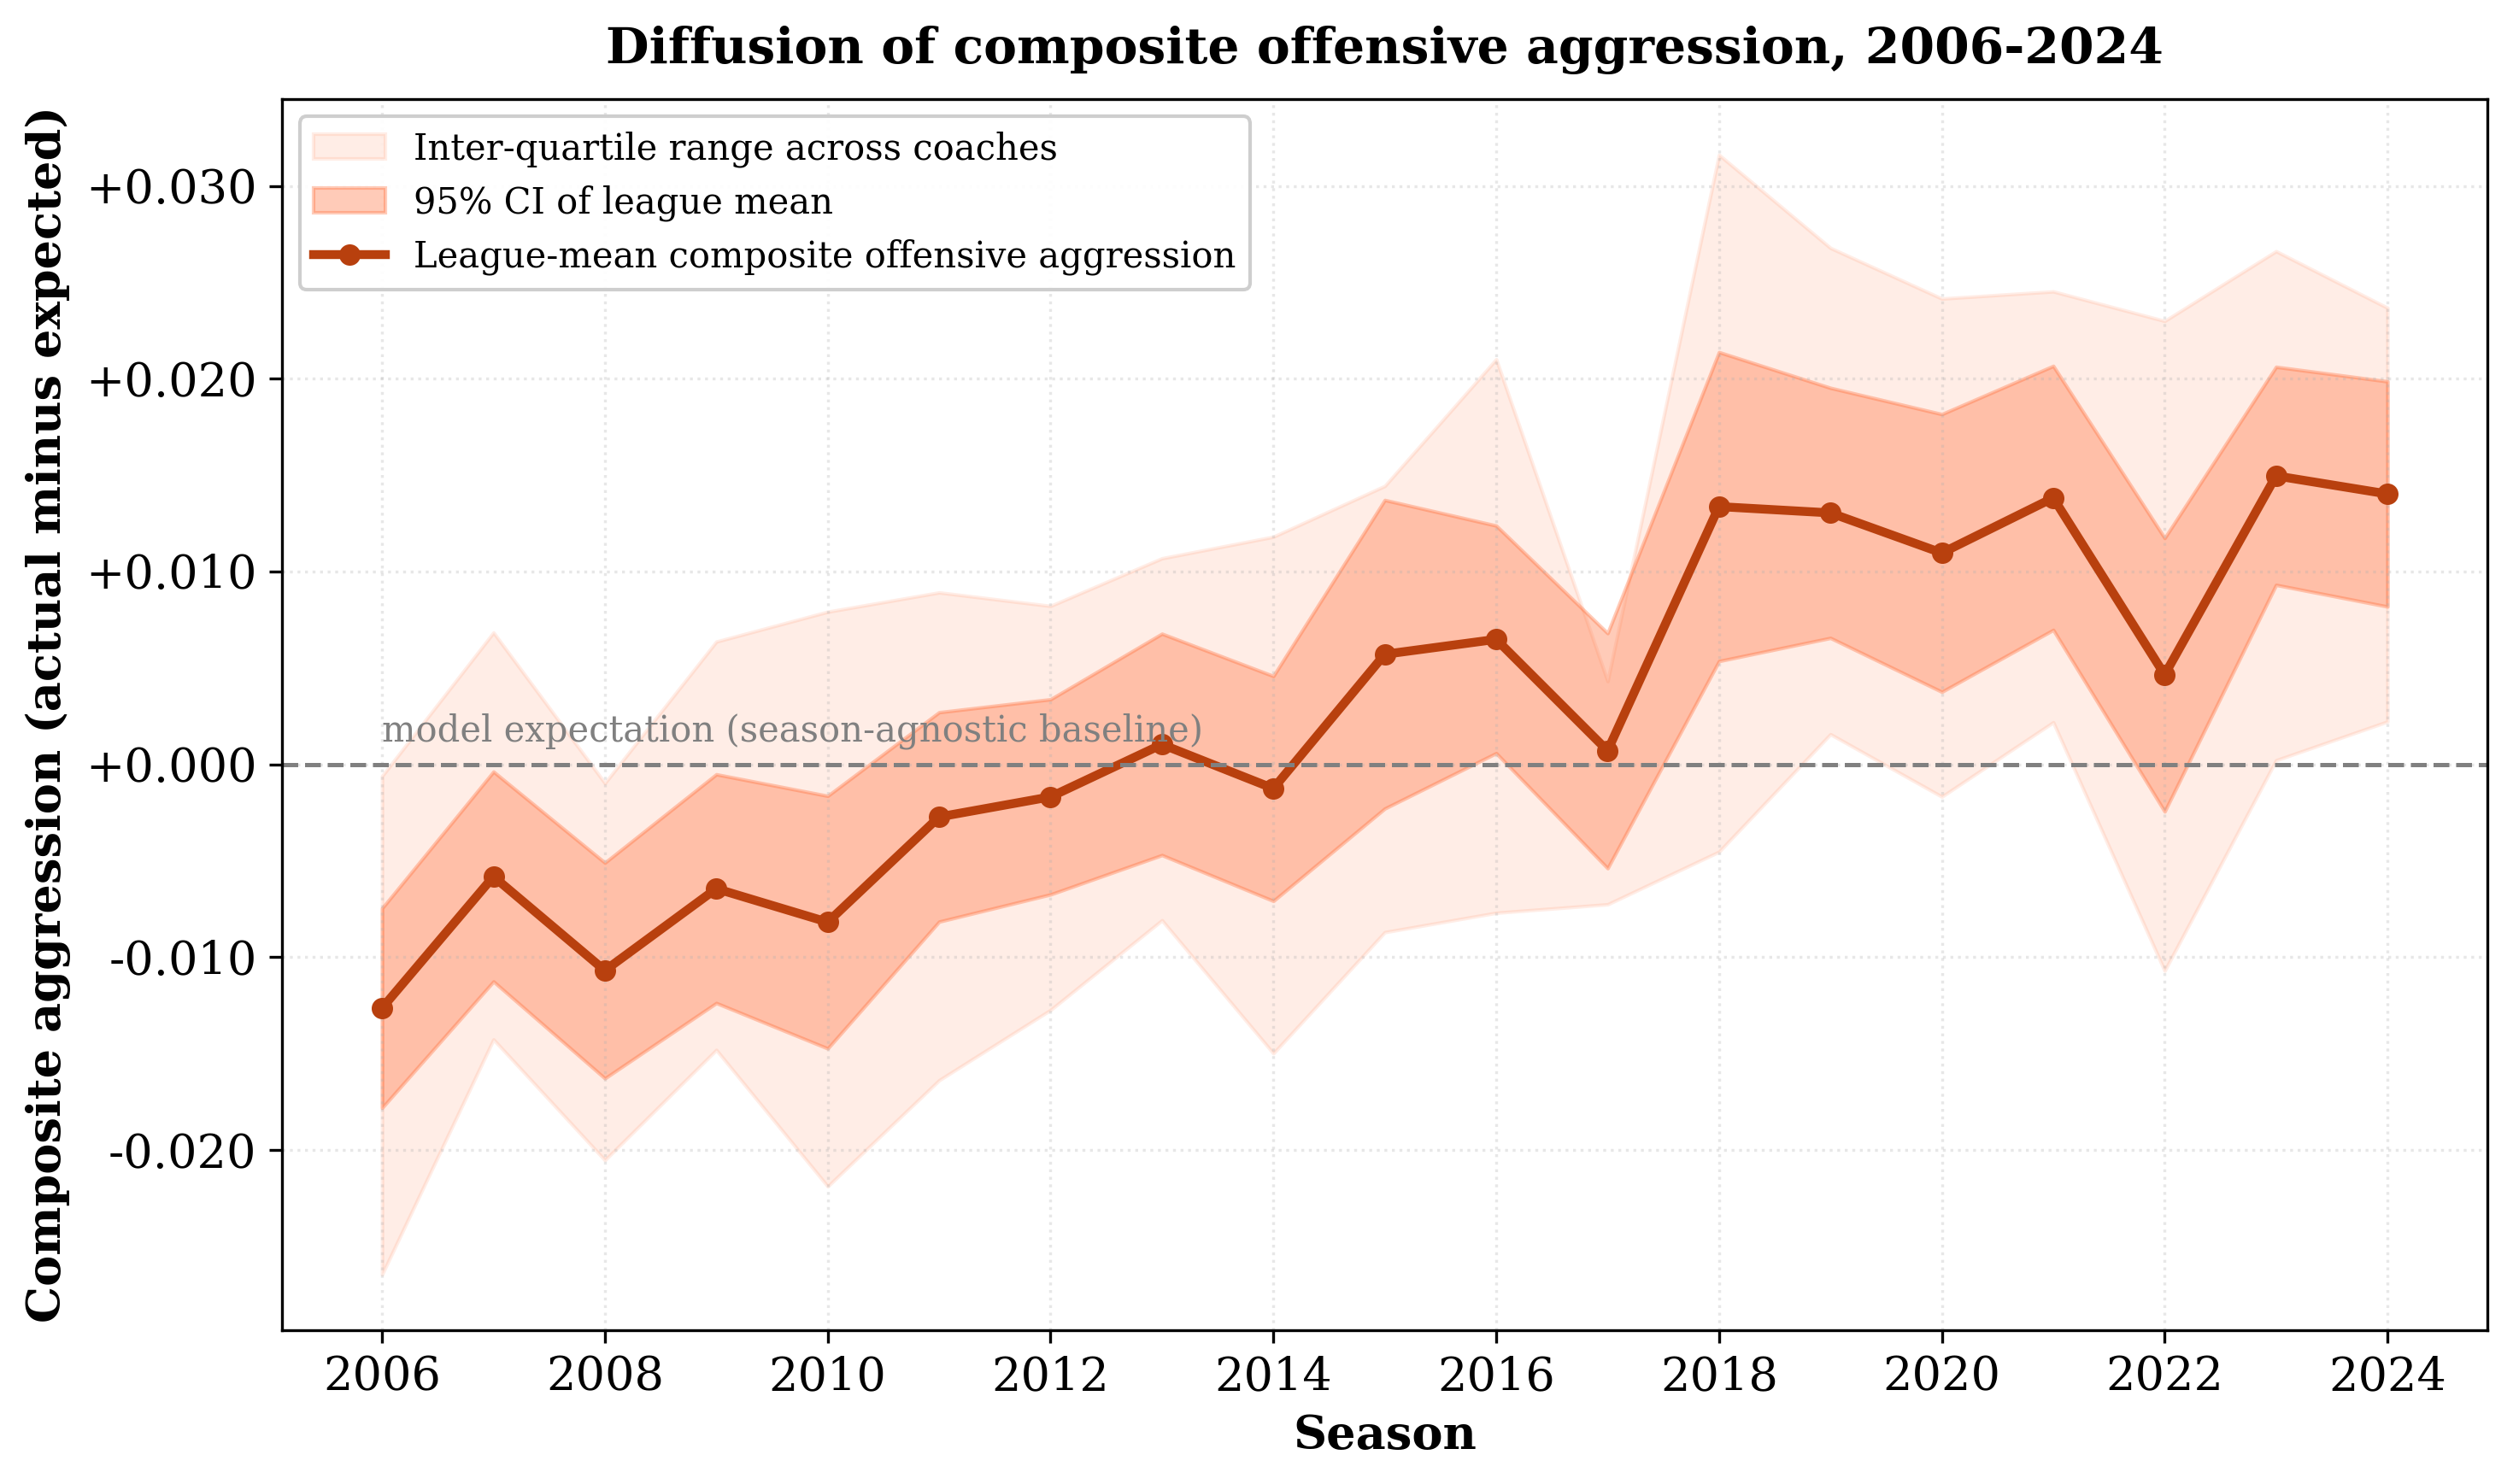
\includegraphics[width=0.82\textwidth]{../../visualizations/performance/aggression_adoption_curve.png}
\caption{Horizontal diffusion of offensive aggression, 2006--2024. The league-mean
composite gene (deviation from the time-invariant, season-agnostic expectation)
rises from below the baseline in the late 2000s to above it by the early 2020s, the
profile of a payoff-driven tactic copied among contemporaries. Because the
expectation model excludes season, this drift is a horizontal-transmission signal
rather than a modeling artifact; it is the same signal the contemporary-group
adjustment removes in the confirmatory tests.}
\label{fig:adoption}
\end{figure}

\subsection{Defensive aggression: attitude and scheme entangled}
Defensive aggression is the one composite that both transmits ($h^{2}=0.49$) and
predicts winning ($S=0.15$), and it is chiefly why the cross-trait relationship is
not cleanly negative. It is best read not as a counterexample but as a reminder that
our two-family taxonomy, approach versus identity, is cleaner on offense than on
defense. ``Aggression'' on defense bundles two dimensions the offensive split holds
apart. One is genuine attitude, how much risk a defense takes: loading the box,
sending extra rushers. The other is schematic, which system a defense runs: man
versus zone coverage is a system choice as much as operating from shotgun is,
closer to a formation than to a fourth-down gamble. A composite that mixes an
attitudinal dimension with a schematic one inherits some of the transmissibility of
scheme and some of the fitness link of attitude, which is precisely the both-corner
position it occupies. The sub-traits bear this out: box-stacking and pass-rush
transmit strongly ($h^{2}\approx0.43$), like schematic identity, while man coverage
transmits weakly ($h^{2}=0.14$); even within defensive aggression the components do
not behave alike. The organizing distinction is therefore attitude versus scheme,
not offense versus defense, and a cleaner future decomposition would separate a
defense's risk posture from its coverage system.

\subsection{Coaching lineages transmit systems, not success}
The pedigree logic that drives NFL hiring finds little support for its strongest
claim. Working under a successful mentor does not, in these data, predict a
protege's own success (mentor-protege WAR resemblance near zero), and the in-game
risk tendency that does predict success is not passed down. What coaching trees
reliably transmit is schematic system, formation and tempo identity, and
specifically through the coordinator who would install it. There is a labor-market
reading of this asymmetry: an organization can observe and verify the system a
coordinator runs far more readily than whether he will win, so hiring on visible
schematic pedigree is hiring on the trait that transmits, not the trait that drives
value. What is legible (system) and what is decisive (in-game approach) come apart,
and only the former leaves a lineage to point to. We offer this as interpretation
rather than a tested claim; the confirmatory result is the decoupling itself.

\subsection{Limitations}
The transmission samples are small (about 40 offensive and 12--17 defensive
coordinator-to-head-coach transitions), so the $h^{2}$ posteriors are wide and the
cross-trait test in particular has low power; H3's wide interval should be read as
inconclusive about a weak relationship, not as evidence for a positive one.
Coaching pedigrees are non-tree, with multiple simultaneous mentors and overlapping
careers, and coaching relatedness can only be assumed by analogy rather than
derived from a Mendelian process, so we use a parent-offspring regression rather
than a pedigree animal model. The genes attribute team play-calling to the head
coach and do not isolate a coordinator's individual contribution; the transmission
tests therefore ask whether the head-coaching style a coach apprenticed under
predicts his own later style, a mentor-protege resemblance that is consistent with
social learning but cannot on its own be separated from assortative hiring, in
which head coaches recruit coordinators who already share their approach. We
therefore read $h^{2}$ as vertical transmissibility in the broad sense. The
defensive-aggression measures begin in 2016 and man coverage in 2018, and the
defensive-aggression to WAR link may partly reflect reverse causation (better
defensive talent enables man coverage and extra rushers). Finally, single-season
WAR is noisy; we address this with inverse-variance weighting and treat the
season-level estimates as conservative floors.

\subsection{Conclusion}
Treating the NFL coaching tree as a cultural pedigree, we find that the strategic
traits that transmit are largely not the traits that win. Schematic identity is
inherited but neutral; offensive aggression is selected but personal and,
strikingly, not heritable despite being a stable individual trait; defensive
aggression alone both transmits and wins. The negative heritability-fitness
relationship of biological populations does not appear; transmission and selection
are instead decoupled, and the fitness-linked behavior spreads horizontally rather
than down the lineage. Coaching trees, in the end, propagate systems, not success.

%% ----------------------------------------------------------------------------
\section*{Supplementary material}

\begin{table}[h]
\centering
\caption{Within-era phylogenetic signal on the mentor network (Moran's $I$ on a
row-normalized, undirected adjacency of mentor--protege ties; one-sided permutation
$p$ from within-career-midpoint-era label shuffles). $E[I]=-1/(N-1)$ is the
no-signal expectation. Under the exploratory Benjamini--Hochberg correction the
defensive-aggression and tempo signals survive.}
\label{tab:moran}
\begin{tabular}{lcccccc}
\toprule
Gene & $I$ & $E[I]$ & $z$ & $p$ & $N$ & edges \\
\midrule
Offensive aggression & $-0.01$ & $-0.01$ & $-0.04$ & 0.52 & 139 & 440 \\
Shotgun & $+0.08$ & $-0.01$ & $+1.77$ & 0.04 & 139 & 440 \\
Tempo & $+0.12$ & $-0.01$ & $+2.63$ & 0.008 & 139 & 440 \\
Defensive aggression & $+0.21$ & $-0.01$ & $+3.03$ & 0.002 & 95 & 216 \\
\bottomrule
\end{tabular}
\end{table}

%% ----------------------------------------------------------------------------
\section*{Acknowledgments}
This work uses play-by-play data from \texttt{nfl\_data\_py} and coaching histories
from Pro Football Reference; the WAR phenotype is from the companion Coach\_WAR
project.

%% ----------------------------------------------------------------------------
\begin{thebibliography}{99}

\bibitem[Benjamini and Hochberg(1995)]{benjamini1995}
Benjamini, Y., \& Hochberg, Y. (1995). Controlling the false discovery rate.
\textit{Journal of the Royal Statistical Society: Series B}, 57(1), 289--300.

\bibitem[Boyd and Richerson(1985)]{boydricherson1985}
Boyd, R., \& Richerson, P. J. (1985). \textit{Culture and the Evolutionary
Process}. University of Chicago Press.

\bibitem[Cavalli-Sforza and Feldman(1981)]{cavallisforza1981}
Cavalli-Sforza, L. L., \& Feldman, M. W. (1981). \textit{Cultural Transmission and
Evolution: A Quantitative Approach}. Princeton University Press.

\bibitem[DerSimonian and Laird(1986)]{dersimonian1986}
DerSimonian, R., \& Laird, N. (1986). Meta-analysis in clinical trials.
\textit{Controlled Clinical Trials}, 7(3), 177--188.

\bibitem[Falconer and Mackay(1996)]{falconermackay1996}
Falconer, D. S., \& Mackay, T. F. C. (1996). \textit{Introduction to Quantitative
Genetics} (4th ed.). Longman.

\bibitem[Fisher(1930)]{fisher1930}
Fisher, R. A. (1930). \textit{The Genetical Theory of Natural Selection}. Clarendon
Press.

\bibitem[Henrich(2016)]{henrich2016}
Henrich, J. (2016). \textit{The Secret of Our Success: How Culture Is Driving Human
Evolution, Domesticating Our Species, and Making Us Smarter}. Princeton University
Press.

\bibitem[Kimura(1968)]{kimura1968}
Kimura, M. (1968). Evolutionary rate at the molecular level. \textit{Nature},
217(5129), 624--626.

\bibitem[Kruuk et al.(2000)]{kruuk2000}
Kruuk, L. E. B., Clutton-Brock, T. H., Slate, J., Pemberton, J. M., Brotherstone,
S., \& Guinness, F. E. (2000). Heritability of fitness in a wild mammal population.
\textit{Proceedings of the National Academy of Sciences}, 97(2), 698--703.

\bibitem[Mesoudi(2020)]{mesoudi2020}
Mesoudi, A. (2020). Cultural evolution of football tactics: strategic social
learning in managers' choice of formation. \textit{Evolutionary Human Sciences},
2, e25.

\bibitem[Moran(1950)]{moran1950}
Moran, P. A. P. (1950). Notes on continuous stochastic phenomena.
\textit{Biometrika}, 37(1/2), 17--23.

\bibitem[Mousseau and Roff(1987)]{mousseauroff1987}
Mousseau, T. A., \& Roff, D. A. (1987). Natural selection and the heritability of
fitness components. \textit{Heredity}, 59(2), 181--197.

\bibitem[Nakagawa and Schielzeth(2010)]{nakagawa2010}
Nakagawa, S., \& Schielzeth, H. (2010). Repeatability for Gaussian and non-Gaussian
data. \textit{Biological Reviews}, 85(4), 935--956.

\bibitem[Price(1970)]{price1970}
Price, G. R. (1970). Selection and covariance. \textit{Nature}, 227(5257),
520--521.

\bibitem[Williamson(2026)]{williamson2026war}
Williamson, J. (2026). Coach WAR: a counterfactual approach to evaluating NFL head
coach impact in the modern era. Companion manuscript.

\bibitem[Wilson et al.(2010)]{wilson2010}
Wilson, A. J., Reale, D., Clements, M. N., Morrissey, M. M., Postma, E., Walling,
C. A., Kruuk, L. E. B., \& Nussey, D. H. (2010). An ecologist's guide to the animal
model. \textit{Journal of Animal Ecology}, 79(1), 13--26.

\end{thebibliography}

\end{document}
